%Memory
Increase in computational power of most state-of-the-art systems has resulted in memory bottlenecks becoming a more and more important from the point of view of performance and energy constraints in the system.
In this section, we briefly describe the role that memory design has to play in our vision-based accelerator system.

\subsection{Motivation}
Memory is an important component of almost all computer-based systems. Given the increase in cloud-computing and server farms, the scalability in terms of power and performance of memory devices has become an important design consideration. Due to it's low-cost per bit, the dynamic random-access memory (DRAM) has become ubiquitous in most commercial applications. However as densities increase, the power wall is becoming an increasingly severe problem. Figure~\ref{fig:refreshTrends} shows the increasing power consumption across different DRAM densities. More crucially, the refresh component in the DRAM is becoming a major source of concern. 
Considerable work has gone into the area of reducing refresh power consumptions. Some have used scheduling policies~\cite{Stuecheli2010}, some have used retention profiling~\cite{Liu2012}, while others have used software techniques~\cite{Liu2012}. In~\cite{Nair2013}, the authors use a refresh pausing mechanism to exploit idle cycles in memory. In~\cite{Mukundan2013}, Fine Grained Refresh (FGR) for DDR4 DRAM systems is analyzed.  

%\begin{figure}[ht!]
%\centering
%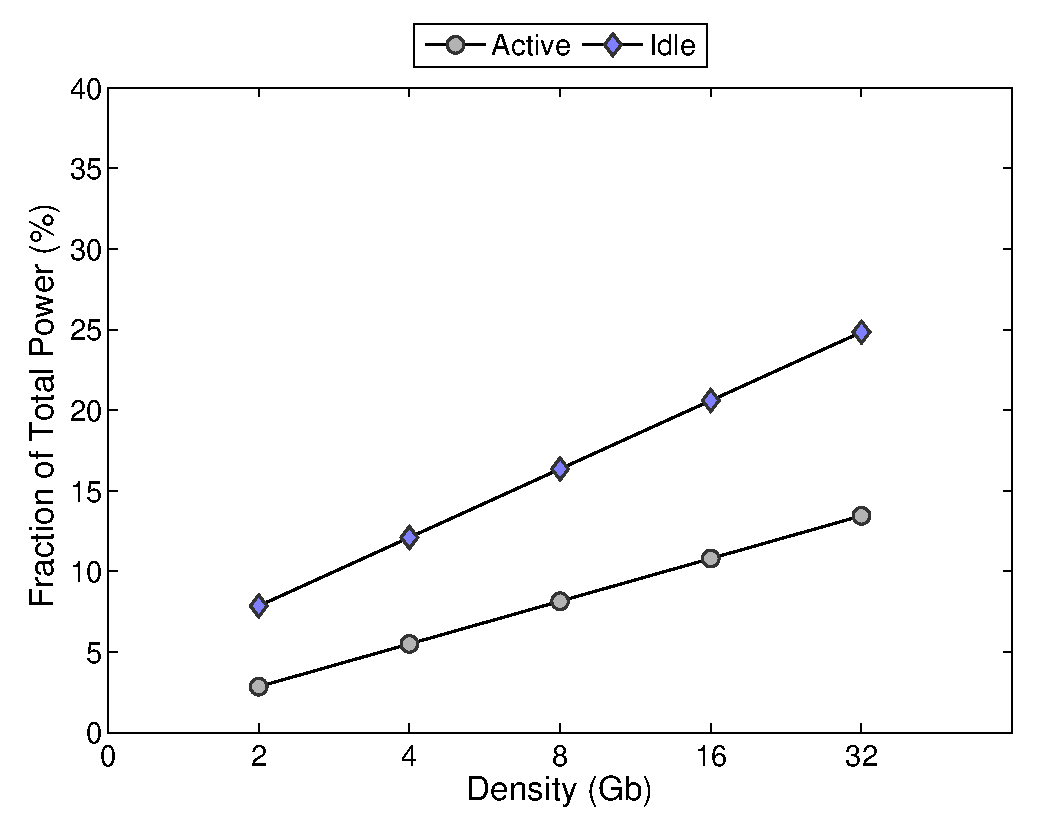
\epsfig{file=figs/RefreshTrends.eps, angle=0, width=1\linewidth, clip=}
%\caption{\label{fig:refreshTrends} Trends in the distribution of DRAM power- The refresh component increases with each generation.}
%\end{figure}

\begin{figure}[ht!]
\begin{minipage}[b]{1\linewidth}
\centering
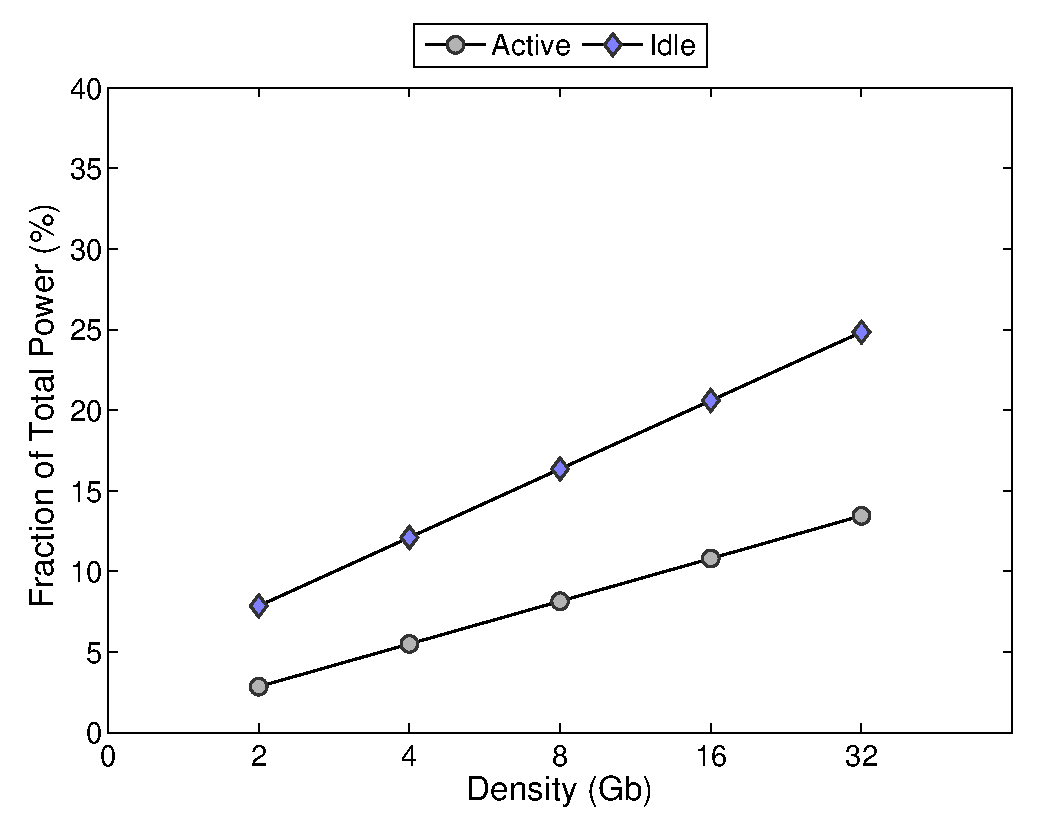
\epsfig{file=figs/RefreshTrends.eps, angle=0, width=1\linewidth, clip=}
\caption{\label{fig:refreshTrends}a) Trends in the distribution of DRAM power- The refresh component increases with each generation.}
\end{minipage}
\begin{minipage}[b]{1\linewidth}
\centering
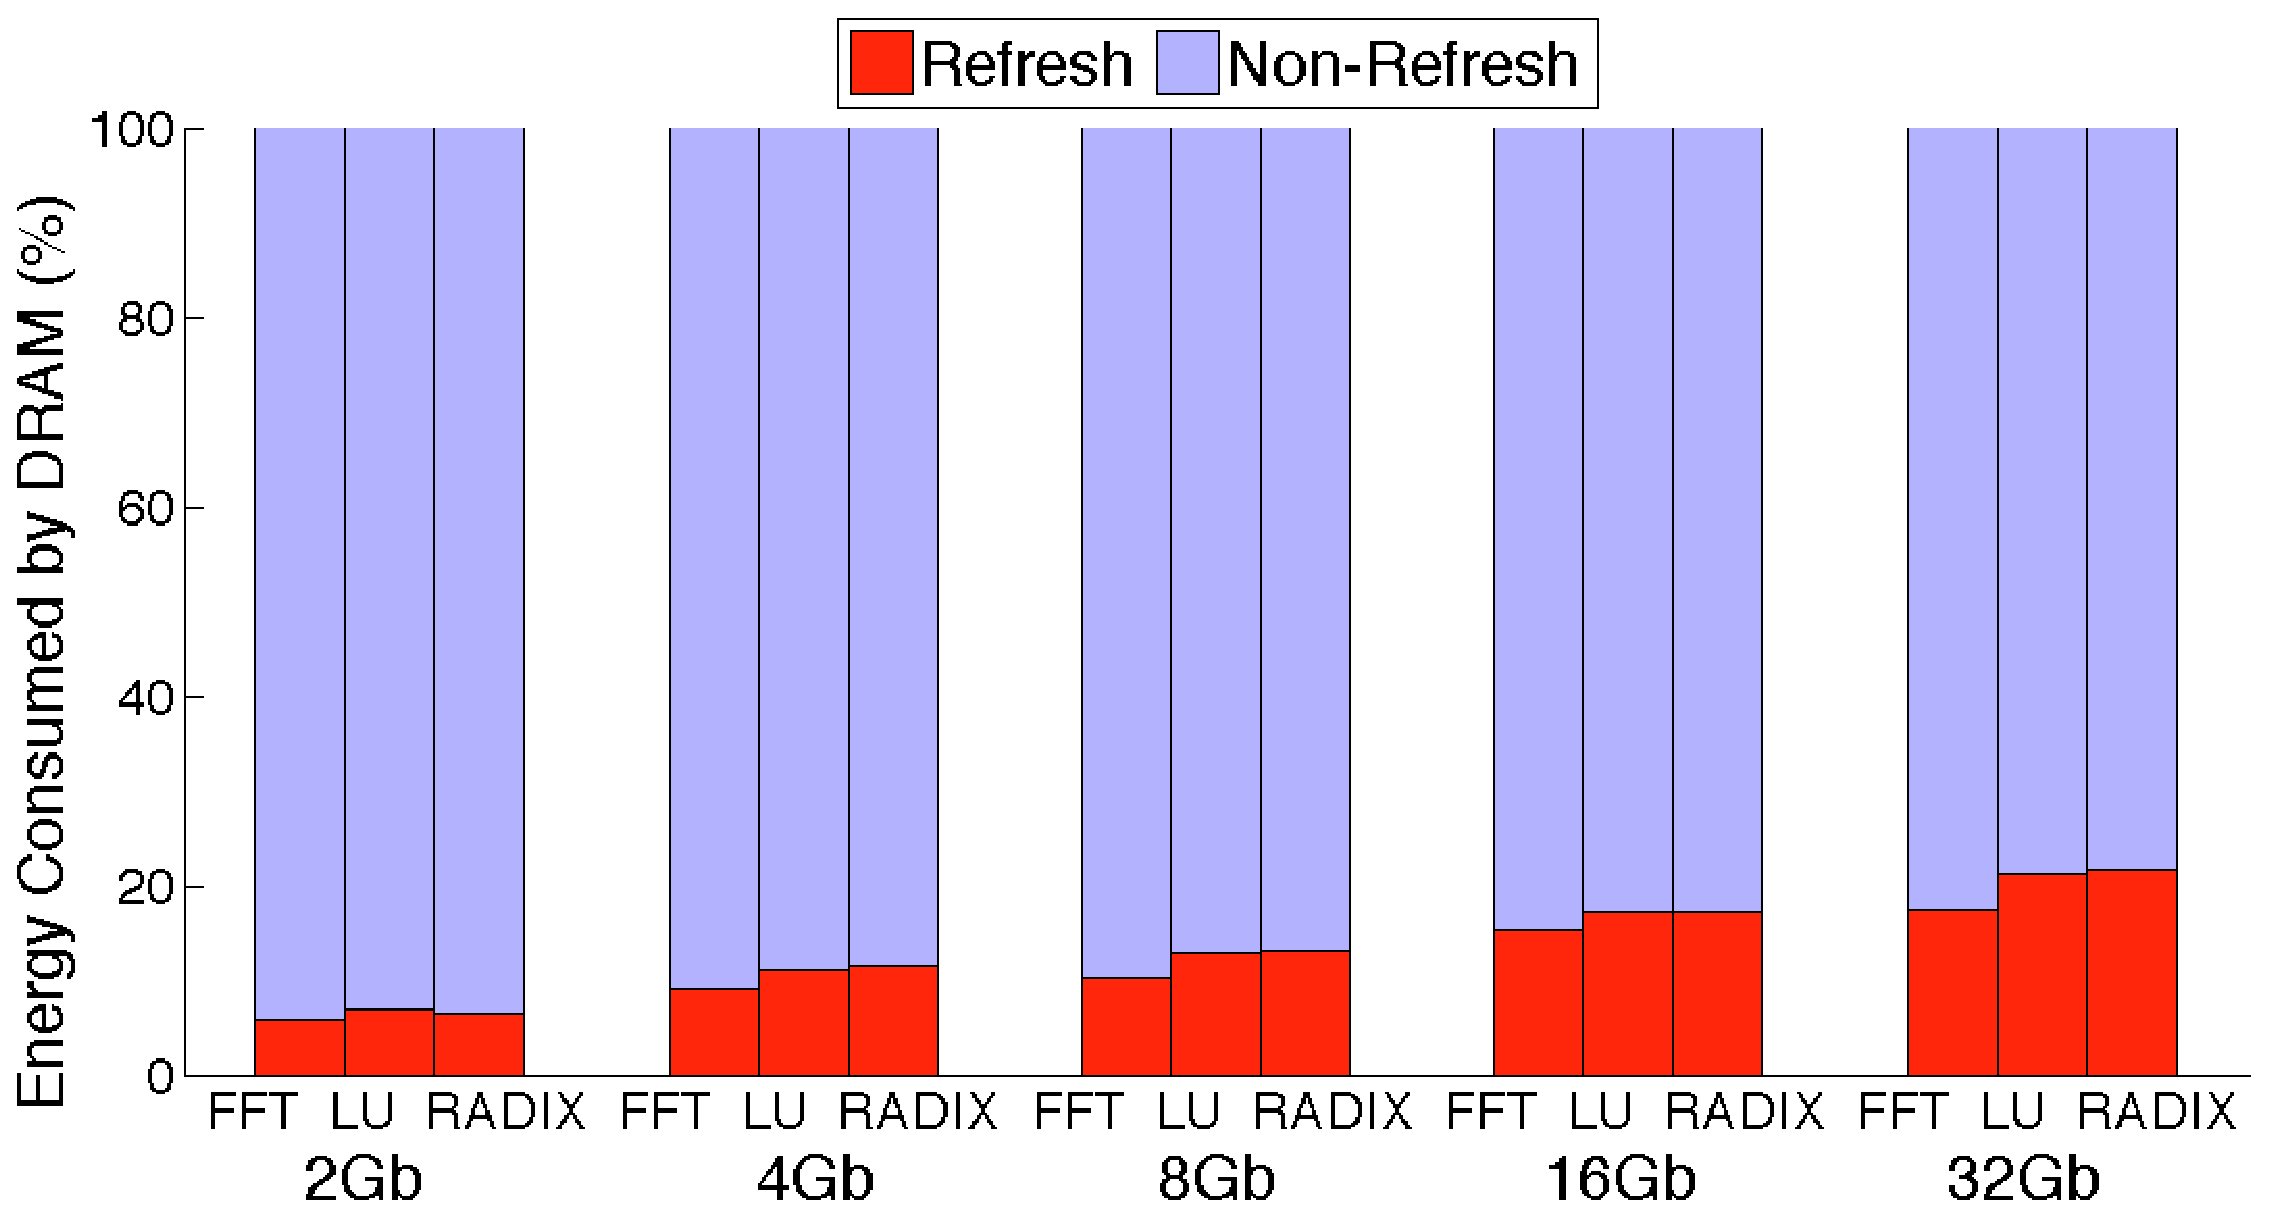
\epsfig{file=figs/DRAMEnergy_Kernels.eps, angle=0, width=1\linewidth, clip=}
\caption{\label{fig:refreshTrends}b) Refresh energy distribution in Kernel computations}
\end{minipage}
%\begin{minipage}[b]{0.25\linewidth}
%\raggedright
%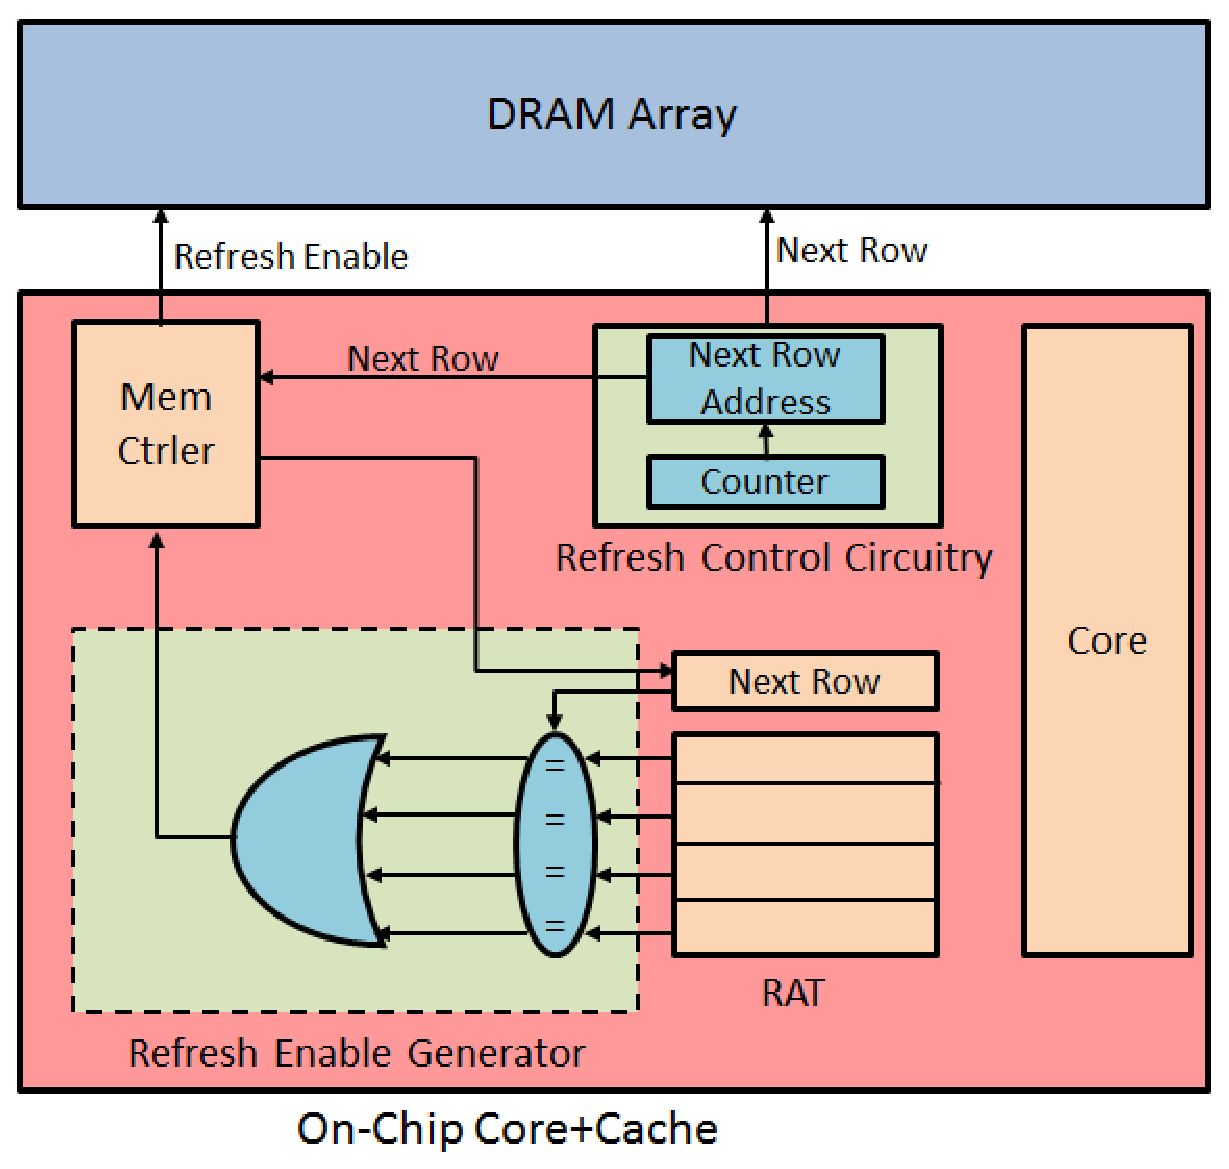
\epsfig{file=figs/refresh_circuitry.eps, angle=0, width=1\linewidth, clip=}
%\caption{\label{fig:reva}c) Design of REVA block}
%\end{minipage}
\end{figure}

\subsection{DRAM Memory Organization}

DRAMs are organized into a series of hierarchical structures in order to exploit the potential for parallelism across accesses. The DRAM consists of one or more memory channels, each one of which has a dedicated memory controller. Each channel comprises of several ranks. Instructions can be issued to the DRAM at the rank level granularity. Each of these ranks are further subdivided into banks. A bank is a logical organization representing an independent memory array and consists of several rows. In general, each row is designed to hold a page of memory (2-4KB).

\subsection{Refresh Operation in DRAMs}
The defining attribute of DRAMs, in comparison to other memory technologies like Static RAMs and Hard Disks is the temporary nature of the data stored in it. Since a DRAM cell simply comprises of a single transistor-capacitor combination, the data is retained for only as long as the capacitor can hold the charge injected into it during a write operation. As a result it is essential to periodically refresh the data in each cell in order to maintain the integrity of the stored data. A refresh operation simply involves reading a row of data and writing it back from the sense amplifier. The write operation restores the charge in each DRAM cell capacitor to its original level. This refresh operation is handled by a built-in refresh controller. The memory controller periodically issues commands to carry out refresh to each rank.

The exact row to be refreshed and the corresponding bank are determined by the refresh controller. Most standard DRAM cells are architected with a 64~ms refresh window ($t_{REFW}$), that is each cell must be refreshed at least once every 64~ms. According to JEDEC SDRAM standards~\cite{jedec-sdram-standards}, a DRAM device can issue a maximum of 8192 refresh commands within this refresh window, leading to a refresh command being issued every 7.8$\mu$s ($t_{REFI}$). Consequently, increasing the number of rows per bank would necessitate multiple rows to be refreshed per command. The refresh controller keeps track of the address of the last row to have been refreshed so that the subsequent refresh command can enable it to issue refreshes to the next group of rows.

The major drawback of DRAM technology is the additional overhead in performance and power on account of the refresh operation. A single refresh command to a row causes the entire bank of the DRAM to stall. Hence several techniques have been incorporated into the DDR protocols to minimize overlaps between read/write and refresh commands.

Each refresh command issued by the memory controller is appended to the command queue along with other read and write commands. Depending on the read and write traffic, it is possible to delay the refresh commands so as to reduce stalls due to the refresh operation preventing the read or write from being issued to the memory. 

